\documentclass[10pt, a4paper]{article}

\usepackage[utf8]{inputenc}
\usepackage{graphicx}
\graphicspath{ {images/} }
\usepackage{mathtools}
\usepackage{amssymb}
\usepackage{amsmath}
\usepackage[english, ngerman]{babel}
\usepackage{cite}
\usepackage{bibgerm}
\usepackage{fullpage}
\usepackage[top=1.5cm,bottom=1.5cm,left=3.5cm,right=2.5cm,headsep=1.5cm,includeheadfoot]{geometry}
\usepackage{tabularx}
\usepackage{caption}
\usepackage{subcaption}
\usepackage{eurosym}
\usepackage{enumitem}
\usepackage{multicol}
\usepackage{tikz}
\usepackage{tkz-euclide}
\usepackage{pgfplots}
\usepackage{pdflscape}
\usepackage{acronym}
\usepackage{blindtext}
\usepackage{ifthen}
\usepackage{setspace}
\usepackage{cancel}
\usepackage{color}
\usepackage{listings}
\usepackage{comment}
\usepackage{xcolor}
\usepackage{colortbl}
\usepackage[parfill]{parskip}

\usepackage{fancyhdr}
\pagestyle{fancy}

\fancyhf{} % clear all
\fancyhead[L]{\leftmark}
\fancyfoot[C]{-- \thepage{} --}
%\setlength{\headheight}{15pt}
\renewcommand{\headrulewidth}{0.5pt}
\renewcommand{\footrulewidth}{0pt}
\setlength{\skip\footins}{0.7cm}

\usetikzlibrary{graphs}
\usetikzlibrary{positioning}

\onehalfspacing
\setlength\parindent{0pt}

%\everymath{\displaystyle}

\allowdisplaybreaks

\definecolor{AI-BLUE}{rgb}{0,0.57,0.87}

% Eigene Befehle
\newcommand\q[1]{\glqq{}#1\grqq{}}
\renewcommand\equiv{\Leftrightarrow}
\newcommand\vertequal[2]{\underset{\underset{#2}{\parallel}}{#1}}
\newcommand\cif{\text{if }}
\newcommand\abs[1]{\left|#1\right|}
\newcommand\norm[1]{\abs{\abs{#1}}}
\newcommand\diff[1]{\text{ d#1}}
\newcommand\av[1]{\left\langle#1\right\rangle}
\newcommand\ev[1]{\mathbb{E}\left(#1\right)}
\newcommand\br[1]{\left(#1\right)}
\newcommand\ubr[2]{\underbrace{#1}_{#2}}
\newcommand\quer[1]{\overline{#1}}
\newcommand\setequal{\overset{!}{=}}
\newcommand\dint{\displaystyle \int}
\newcommand\dsum{\displaystyle \sum}
\newcommand\dprod{\displaystyle \prod}
\newcommand\closedInt[2]{\left[#1,#2\right]}
\newcommand{\checkbox}{\Large \Square \normalsize \hspace{0.4cm}}

\newcommand\myref[1]{\ref{#1} (S. \pageref{#1})}
\newcommand\myrefcomma[1]{\ref{#1}, S. \pageref{#1}}

\newcommand\nsm{Nagel-Schreckenberg-Modell }

\begin{document}

\thispagestyle{empty}

\setlength{\hoffset}{-0.5cm} % center title page

\lstset{
  basicstyle=\small,           % the size of the fonts that are used for the code
  breaklines=true,             % sets automatic line breaking
  captionpos=b,                % sets the caption-position to bottom
  frame=single,                % adds a frame around the code
  keepspaces=true,             % keeps spaces in text, useful for keeping indentation of code (possibly needs columns=flexible)
  numbers=right,               % where to put the line-numbers; possible values are (none, left, right)
  showspaces=false,            % show spaces everywhere adding particular underscores; it overrides 'showstringspaces'
  stepnumber=1,                % the step between two line-numbers. If it's 1, each line will be numbered
  tabsize=4,                   % sets default tabsize to 4 spaces
  xleftmargin=0.14cm		   % sets left margin
}


\begin{titlepage}
    \begin{center}
    \vphantom{0cm}
    \LARGE \textbf{Dokumentation}\\
    \vspace{3cm}
    \normalsize
    Dokumentation für Simulationstechnik \\
    im Master-Studiengang \textcolor{AI-BLUE}{[Angewandte Informatik]}\\
    an der Ruhr-Universität Bochum\\
    im Wintersemester 2014/15\\
    \vspace{4cm}
    \huge \textbf{Verkehrssimulation mit Zellularautomaten in C++} \\
    \vspace{4cm}
    \normalsize
    \textbf{Projektteilnehmer:}\\
    B. Sc. Christian Andreas Mielers (108 011 204 956)\\
    B. Sc. Phil Yannick Schrör (108 011 214 024)\\
    \vspace{2cm}
    \textbf{Projektbetreuer:}\\
    M. Sc. Markus Scheffer
    \end{center}
\end{titlepage}

\newpage
\pagenumbering{arabic}
\setcounter{page}{2}

\tableofcontents

\newpage
\section{Einleitung}
\label{sec:einleitung}
Eine umfassende, allgemeingültige Vorhersage von Verkehrsflüssen entzieht sich analytischen Methoden. Dies liegt zum einen an der Vielzahl möglicher, in der Realität relevanter Szenarien und Einflussfaktoren und zum anderen daran, dass die Zustände eines Verkehrssystems nicht gedächtnislos sind, sondern vom vorherigen Zustand abhängen. Dies macht die Simulation des Verkehrsflusses auf Basis von Eingangsgrößen und Parametern zu einer attraktiven Alternative. Wir beschäftigen uns im Folgenden mit der Simulation dreier Szenarien: Einer einspurigen und einer mehrspurigen Autobahn sowie einem Kreisverkehr. Zunächst beschreiben wir die von uns getroffenen Annahmen. Anschließend gehen wir auf die Umsetzung ein, wobei es für einspurige und zweispurige Autobahnen bereits etablierte Verfahren auf Basis zellulärer Automaten gibt, für den Kreisverkehr haben wir jedoch ein eigenes Verfahren entwickelt. Wir werden sehen, dass sich unser für den Kreisverkehr entworfenes Verfahren aufgrund seiner Generalität auf beliebige Straßennetze anwenden lässt. Aufgrund der Komplexität des Systems haben wir uns dazu entschlossen, die Implementierung in C++ vorzunehmen\footnote{Dies erfolgte in Absprache mit unserem Betreuer.}. Abschließend bestimmen wir verschiedene Parameter, bei denen es zu Verlangsamungen und Staus im Verkehrsfluss kommt.

\section{Annahmen}
\label{sec:annahmen}

Im Groben basiert unser Modell auf den Annahmen, die Kai Nagel und Michael Schreckenberg \cite{nagel-schreckenberg} für ihr STCA-Verkehrsmodell (STCA = Standard Zellular-Automat) getroffen haben. Um das Modell an die Realität deutscher Straßenverhältnisse anzupassen, wurden jedoch einige Änderungen vorgenommen.
Im Folgenden werden die unserem Modell zugrunde liegenden Annahmen aufgeführt.

\subsection{Zellgröße und Geschwindigkeiten}

Es gilt weiterhin, dass jede Zelle 7,5 Meter lang ist und nur ein einziges Fahrzeug zur gleichen Zeit aufnehmen kann.

Im klassichen \nsm gibt es die Geschwindigkeitsstufen 0 bis 5. Diese entsprechen Geschwindigkeiten von 0 $km/h$ bis 135 $km/h$ in 27 $km/h$ Abständen. Da uns 135 $km/h$ als Höchstgeschwindigkeit auf einer deutschen Autobahn zu wenig erschienen, haben wir die Höchstgeschwindigkeit auf 7 erhöht, so dass Fahrzeuge nun eine Maximalgeschwindigkeit von 189 $km/h$ erreichen können.

Während im \nsm alle Fahrzeuge üblicherweise die gleiche Maximalgeschwindigkeit erreichen können, werden in unserem Modell die Maximalgeschwindigkeiten der Fahrzeuge aus einer Normalverteilung gezogen, deren Mittelwert und Standardabweichung vom Nutzer des Programms frei gewählt werden können. Wir halten dieses Szenario für realistischer, da in der Realität unterschiedliche Fahrzeugtypen unterschiedliche Maximalgeschwindigkeiten erreichen können. Es ist zu beachten, dass es nicht möglich ist, auf diese Weise Fahrzeugen Maximalgeschwindigkeiten unter 3 oder über 7 zuzuweisen, da in Deutschland nur solche Fahrzeuge eine Autobahn befahren dürfen, welche eine Höchstgeschwindigkeit von mindestens 60 $km/h$ erreichen können. Ein Fahrzeug mit der Höchstgeschwindigkeit 2 (= 54 $km/h$) wäre $6km/h$ zu langsam.

\subsection{Individuelles Fahrverhalten}

Um das Fahrverhalten unterschiedlicher Fahrertypen abbilden zu können, wird der Trödelfaktor eines jeden Fahrzeugs randomisiert bestimmt. Zu diesem Zweck wird jedoch keine Normalverteilung verwendet, sondern eine Gleichverteilung, deren Minimalwert und Maximalwert ebenfalls frei vom Nutzer festgelegt werden können (es gelten die natürlichen Schranken 0 und 1). Ist keine Varianz erwünscht, kann durch Gleichsetzung von Minimal- und Maximalwert ein konstanter Trödelfaktor definiert werden.

Über eine Maximalgeschwindigkeit und einen Trödelfaktor hinaus hat in unserem Modell jedes Fahrzeug zwei individuelle Risikofaktoren. Diese dienen auf der Autobahn als Wahrscheinlichkeit dafür, ohne Rücksicht auf Abstände auf die Spur links bzw. rechts zu wechseln. Es ist notwendig zwei Risikofaktoren zu verwenden, da Fahrer je nach individuellem Fahrverhalten oft dazu neigen, tendenziell nach links oder tendenziell nach rechts zu fahren. Ein Fahrer, der möglichst schnell vorwärts kommen möchte, riskiert es eher, nach links zu fahren als nach rechts. Bei Fahrern, die auf das Rechtsfahrgebot achten oder sich unsicher auf der Autobahn fühlen, verhält es sich eher anders herum.

Da wir annehmen, dass die Mehrheit der Fahrer eher rücksichtsvoll ist und weniger Fahrer riskante Fahrmanöver unternehmen, ziehen wir die Riskofaktoren aus Exponentialverteilungen. Die linke Seite der folgenden Abbildung zeigt eine mögliche Dichtefunktion für den Risikofaktor L2R (Wechsel von links nach rechts), die rechte Seite eine mögliche Dichtefunktion für den Risikofaktor R2L (Wechsel von rechts nach links).

\begin{figure}[h!]
    \centering
    \begin{tikzpicture}[xscale=4, yscale=0.3]
        \def\LAMBDA{12}
        \draw[->] (-0.1,0) -- (1.1,0) node[right] {L2R};
        \draw[->] (0,-0.1) --(0,15) node[above] {Exp($\lambda$ = \LAMBDA)};
        \foreach \x in {0.2,0.4,0.6,0.8,1} {
            \draw[shift={(\x,0)},color=black] (0pt,8pt) -- (0pt,-8pt) node[below] {\x};
        }
        \draw[domain=0:1,samples=800,variable=\x,blue] plot ({\x},{\LAMBDA * exp(- \LAMBDA * \x)});
    \end{tikzpicture}
    \begin{tikzpicture}[xscale=4, yscale=0.3]
        \def\LAMBDA{8}
        \draw[->] (-0.1,0) -- (1.1,0) node[right] {R2L};
        \draw[->] (0,-0.1) --(0,15) node[above] {Exp($\lambda$ = \LAMBDA)};
        \foreach \x in {0.2,0.4,0.6,0.8,1} {
            \draw[shift={(\x,0)},color=black] (0pt,8pt) -- (0pt,-8pt) node[below] {\x};
        }
        \draw[domain=0:1,samples=800,variable=\x,blue] plot ({\x},{\LAMBDA * exp(- \LAMBDA * \x)});
    \end{tikzpicture}
    \caption{Dichtefunktionen der Risikofaktor-Verteilungen}
    \label{fig:riskFactorDistributions}
\end{figure}

Da die Exponentialverteilung nach rechts nicht begrenzt ist, wir jedoch die Begrenzung des Risikofaktors für sinnvoll halten, wird der Risikofaktor auf das 0.97-Fraktil der Verteilung gesetzt, falls genau dieses Fraktil überschritten wird. Bei der in Abbildung \ref{fig:riskFactorDistributions} linken Verteilung mit $\lambda = 12$ beträgt der maximal zulässige Wert also ungefähr 0.2922, während er bei der rechten Verteilung mit $\lambda = 8$ etwa 0.4383 beträgt. In diesem Szenario wären die Fahrer im Durchschnitt eher dazu bereit, ohne Rücksicht auf die Abstände von rechts nach links zu wechseln als umgekehrt.

\section{Umsetzung}
\label{sec:umsetzung}

\subsection{Autobahn}
\label{subsec:umsetzung-autobahn}

Wir haben unser Modell strukturell für die Simulation von Autobahnen mit beliebig vielen Spuren ausgelegt. Die in der Aufgabenstellung unterschiedenen Simulationsexperimente einer einspurigen bzw. einer zweispurigen Autobahn können also mit derselben Software durchgeführt werden. Im Folgenden wird die Umsetzung dieses allgemeinen Modells beschrieben. In Kapitel \ref{sec:ergebnisse} werden selbstredend die Ergebnisse für beide Experimente aufgeführt.

Als Repräsentation für die Autobahn dient eine $l \times s$ Matrix, wobei $l$ die Anzahl der Spuren (engl. \emph{lanes}) und $s$ die Anzahl der Straßensegmente (engl. \emph{segments}) angibt. Für die Simulation einer 2,25km ($= 300 \cdot 7.5m$) langen Autobahn mit drei Spuren wird also eine $3 \times 300$ Matrix erzeugt. Im Wesentlichen dient diese Matrix dazu, Fahrzeuge und ihre Position auf der Autobahn zu speichern.\\

%\begin{figure}[h!]
%	\centering
%	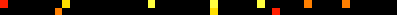
\includegraphics[width=0.8\textwidth]{img/twoLaneRoad}
%	\caption{Zweispurige Autobahn mit unterschiedlich schnellen Fahrzeugen (Ausschnitt)}
%	\label{fig:twoLaneRoad}
%\end{figure}

Im \nsm gibt es Szenarien mit zyklischen und offenen Randbedingungen. Da zyklische Autobahnen weniger realitätsnah sind, haben wir die Simulation zunächst so implementiert, dass stets auf der linken Seite neue Fahrzeuge erzeugt werden und diese bei Verlassen des rechten Randes wieder vernichtet werden. Da es bei dieser Implementierung aber schwierig ist, die Verkehrsdichte auf dem gewünschten Niveau zu halten, wurde zusätzlich eine Implementierung mit periodischen Randbedingungen umgesetzt. Die Entscheidung über die Periodizität der Autobahn wird dem Nutzer des Programms überlassen.

\subsubsection{Initialisierung}
\label{subsubsec:initialisierung}

Dem Nutzer obliegt die Entscheidung, ob zum Start der Simulation Fahrzeuge auf der Autobahn platziert werden oder nicht. Da bei periodischen Randbedingungen keine Fahrzeuge erzeugt (oder vernichtet) werden, ist hier eine Initialisierung notwendig. Ohne periodische Randbedingungen werden in jedem Simulationsschritt mit einer gewissen Wahrscheinlichkeit neue Fahrzeuge erzeugt, so dass eine Initialisierung nicht konzeptionell erforderlich (aber möglich) ist. Um Staus zu vermeiden, die aus einer ungünstigen Initialbelegung hervorgehen, kann der Nutzer entscheiden, ob er die Fahrzeuge zufällig oder äquidistant auf der Autobahn verteilen möchte.
Ausschlaggebend für die Anzahl der erzeugten Fahrzeuge ist die vom Nutzer festgelegte Verkehrsdichte (engl. \emph{traffic density}). Diese kann Werte zwischen 0 (leere Fahrbahn) und 1 (jede Zelle enthält ein Fahrzeug) annehmen. Die Geschwindigkeit des Fahrzeugs wird gesetzt auf das Minimum aus seiner Maximalgeschwindigkeit und dem Abstand zum nächsten vorausfahrenden Fahrzeug. Werden die Fahrzeuge hingegen zufällig auf der Autobahn platziert, wird auf jeder Zelle mit Wahrscheinlichkeit $p =$ \emph{Verkehrsdichte} ein Fahrzeug mit beliebiger Geschwindigkeit zwischen 0 und seiner Maximalgeschwindigkeit erzeugt.

Nachdem die Autobahn initialisiert wurde, wird der Simulationsschritt in einer Schleife ausgeführt. Die einzelnen Teilschritte eines Simulationsschritts werden im Folgenden detailiert behandelt.


\subsubsection{Neue Fahrzeuge hinzufügen}
\label{subsubsec:neueFahrzeuge}

Falls die Simulation mit offenen Randbedingungen durchgeführt wird, ist es notwendig, neue Fahrzeuge zu erzeugen, um die Ausfahrenden zu ersetzen. Bei der Erzeugung neuer Fahrzeuge wird in jedem Simulationsschritt geprüft, ob die aktuelle Verkehrsdichte geringer ist als die angegebene Wunschverkehrsdichte. Ist dies der Fall, wird beginnend mit der rechtesten Spur über alle Spuren iteriert und genau dann in die jeweils erste Zelle ein Fahrzeug eingefügt, wenn diese frei ist und die gewünschte Verkehrsdichte noch nicht erreicht ist.

\subsubsection{Beschleunigen}
\label{subsubsec:beschleunigen}

Die Regeln für die Beschleunigung sind unverändert geblieben. Falls ein Fahrzeug seine Maximalgeschwindigkeit noch nicht erreicht hat, wird seine Geschwindigkeit um eine Stufe erhöht.

\subsubsection{Fahrstreifen wechseln}
\label{subsubsec:fahrstreifenWechseln}

Bei den Regeln für den Fahrstreifenwechsel haben wir uns an den im Anhang von \cite{mehrspurig} aufgeführten \emph{\q{STCA-Regeln für den Fahrstreifenwechsel auf mehrstreifigen Richtungsfahrbahnen}} orientiert. Gemäß diesen Regeln hat ein Fahrzeug den Wunsch auf die Spur links von ihm zu wechseln, falls es auf der eigenen Spur nicht mit Maximalgeschwindigkeit fahren kann und links von ihm mindestens so viel Platz ist wie auf seiner aktuellen. Falls die Geschwindigkeit des nächsten nachfolgenden Fahrzeugs auf der linken Spur kleiner ist als der Abstand zum betrachteten Fahrzeug, wird der Fahrstreifenwechsel tatsächlich vollzogen.

Ein Wechsel auf die rechtsgelegene Spur wird angestoßen, wenn ein linksfahrendes Fahrzeug einen Abstand zu seinem Vordermann hat, der größer als seine Maximalgeschwindigkeit und auf der rechten Spur mindestens so viel Platz wie auf der aktuellen ist. Dann gibt es keinen Grund, auf der linken Spur zu bleiben. Das Fahrzeug folgt somit dem Rechtsfahrgebot und zieht auf die rechte Spur herüber, falls die Geschwindigkeit des nächsten dort nachfolgenden Fahrzeuges kleiner als der Abstand zu ihm selbst ist.

Zusätzlich kann der Fall eintreten, dass ein Fahrzeug ohne Rücksicht auf Abstände den Fahrstreifen wechseln möchte. Dies ist nur möglich, wenn die entsprechende Zelle auf der Zielspur frei ist. Die Wahrscheinlichkeit eines solchen Risikofahrstreifenwechsels wird durch die Risikofaktoren des betrachteten Fahrzeuges definiert. In jedem Simulationsschritt führt ein Fahrzeug mit dieser Wahrscheinlichkeit einen Risikospurwechsel durch.

Da unser System grundsätzlich für beliebig viele Spuren ausgelegt ist, bleibt noch zu klären, ob zuerst versucht werden soll, von rechts nach links zu wechseln, oder umgekehrt. Da Fahrzeuge zum einen bestrebt sind, das Rechtsfahrgebot einzuhalten, aber sie andererseits auch möglichst schnell vorwärts kommen wollen, wird in jedem Simulationsschritt zufällig entschieden, welcher Wechsel zuerst versucht werden soll. Scheitert dieser, wird der andere Wechsel ausprobiert.

\subsubsection{Abstände prüfen}
\label{subsubsec:abstaendePruefen}
Die Regeln für die Überprüfung der Abstände basieren ebenfalls auf den erweiterten STCA-Regeln. Ist die aktuelle Geschwindigkeit eines Fahrzeugs größer als der Abstand zum nächsten vorausfahrenden Fahrzeug, wird die Geschwindigkeit so weit reduziert, dass keine Auffahrunfälle auftreten. Vorausfahrende Fahrzeuge sind hier all jene, die auf der gleichen oder einer linksseitigen Spur vorweg fahren (wegen des Rechtsüberholverbotes). Diesen Teil des STCA-Regelwerks kritisieren wir, da es so nicht möglich ist, dass zwei Fahrzeuge mit ähnlicher Geschwindigkeit nah hintereinander her fahren. Fährt auf der linken Spur ein Fahrzeug eine Zelle weiter vorne als ein Fahrzeug auf der rechten Spur, muss das rechte Fahrzeug seine Geschwindigkeit auf 0 reduzieren, um Auffahrunfälle unmöglich zu machen. 
Realistischer, aber mit mehr Aufwand für die Kollisionsvermeidung verbunden, wäre die Begrenzung der Geschwindigkeit des rechts fahrenden Fahrzeugs auf die Geschwindigkeit des links fahrenden Fahrzeugs.

\subsubsection{Trödeln}
\label{subsubsec:troedeln}

Wie bereits in Kapitel \ref{sec:annahmen} erläutert, wird für jedes Fahrzeug der Trödelfaktor aus einer Gleichverteilung mit nutzerdefiniertem Minimal- und Maximalwert gezogen. Beide Werte dürfen nicht kleiner als 0 sein und der Minimalwert darf nicht größer als der Maximalwert sein. Die Gleichsetzung beider Werte ist aufgrund der oben dargelegten Annahmen jedoch explizit erlaubt. In jedem Simulationsschritt wird nach dem Prüfen der Abstände mit einer Wahrscheinlichkeit gleich dem Trödelfaktor getrödelt, d.h. die Geschwindigkeit um eine Stufe reduziert. Mit Ausnahme der individuellen Trödelfaktoren handelt es sich also um die gleichen Regeln wie im STCA-Modell.

\subsubsection{Fahrzeuge bewegen}
\label{subsubsec:fahrzeugeBewegen}

Im letzten Schritt müssen die Fahrzeuge noch entsprechend ihrer Geschwindigkeit bewegt werden. Da durch die vorherige Prüfung der Abstände Kollisionen unmöglich sind, genügt es, die Fahrzeuge gemäß ihrer Geschwindigkeitsstufe viele Zellen nach rechts zu bewegen. Falls ein Fahrzeug über den rechten Rand der Autobahn hinaus bewegt wird, wird es im Falle von periodischen Randbedingungen in der entsprechenden Zelle am linken Rand eingefügt. Andernfalls erfolgt die Löschung des Fahrzeugs. 

\subsection{Kreisverkehr (und beliebige Straßenverläufe)}
\label{subsec:umsetzung-kreisverkehr}

\subsubsection{Vorüberlegungen}
\label{subsubsec:kreisverkehrUmsetzungVorueberlegungen}

Ein dritter Teil der Aufgabenstellung bestand darin, den Verkehrsfluss eines Kreisverkehrs zu simulieren. Dies ist ein ungleich schwierigeres Problem, da es hier an einigen Stellen Verzweigungen und Zusammenführungen geben kann, bei denen Kollisionsfreiheit gewährleistet werden muss. Zwar kann man den Spurwechsel auf der mehrspurigen Straße auch als Verzweigung/Zusammenführung betrachten, allerdings weist dieser Gleichmäßigkeit über alle Zellen hinweg auf, d.h. die Regeln können einmalig, relativ zur Zellposition und den Geschwindigkeiten der Fahrzeuge festgelegt werden. Im Kreisverkehr hingegen verhalten sich einige Zellen deutlich anders als andere, beispielsweise hinsichtlich zulässiger Geschwindigkeit oder Anzahl der Richtungen, in die man sich bewegen kann. In diesem Zusammenhang müssen auch Vorfahrtsregeln beachtet werden. Darüber hinaus haben Ereignisse in einer Zelle (z.B. die Entscheidung, eine Ausfahrt zu nehmen) Auswirkungen auf die Handlungsmöglichkeiten der Autos in den umliegenden Zellen. Diese Anforderungen machen einen erheblich dynamischeres Vorgehen bei der Berechnung der Bewegungen der Fahrzeuge erforderlich. Eine Lösung muss also folgende Anforderungen erfüllen:

\begin{enumerate}
	\item Kollisionsfreiheit
	\item Vorfahrtsregeln
	\item Geschwindigkeitsbegrenzungen
\end{enumerate}

Grundsätzlich wäre eine simple Lösung möglich, die die Anforderungen dieses spezifischen Szenarios erfüllt. Hierbei würde man die kritischen Stellen, wie die Zu- und Abfahrtszellen zum/vom Kreisverkehr, gesondert (mit eigener Logik) behandeln. Es ist offensichtlich, dass eine solche Lösung hochgradig abhängig vom der Problemstellung ist und man daher für jedes Szenario manuelle Anpassungen vornehmen muss. Dies ist nicht zufriedenstellend, weswegen wir uns ein Verfahren zum Ziel gesetzt haben, dass von Spezifika des Szenarios unabhängig ist.

Strukturell behalten wir das Layout eines Grids bei, in dem die Zellen der Simulation mit x- und y-Koordinaten gespeichert werden. Dies dient allerdings nur der Vereinfachung der Visualisierung. Konzeptionell besteht unsere Straßenkarte aus losen Zellen, die Verweise auf ihre Vorgänger- und Nachfolgerzellen beinhalten. Somit entspricht das Layout unserer Lösung einem gerichteten, nicht notwendigerweise kreisfreien Graphen.

Zunächst betrachten wir die Anforderung der Kollisionsfreiheit. Es soll analog zum Nagel-Schrecken\-berg Modell \cite{nagel-schreckenberg} erreicht werden, dass in keinem Simulationsschritt eine Zelle von mehr als einem Auto befahren wird. Ein einfacher Weg dies zu erreichen besteht darin, alle Fahrzeuge sequenziell durchzugehen und für jedes die Zellen, die es abfahren möchte, zu markieren. Hier geht man nur soweit, wie das Auto mit seiner aktuellen Geschwindigkeit fahren kann. Dabei wird das Markieren gestoppt, sobald eine Zelle erreicht wird, die bereits von einem anderen Auto markiert wurde. Nachdem alle Fahrzeuge ihren Weg markiert haben, wird für jedes die Anzahl der Markierungen gezählt und seine Geschwindigkeit auf diese Zahl gedeckelt.

Bei diesem Ansatz ergibt sich allerdings das Problem, dass Vorfahrtsregeln missachtet werden. Wird zuerst ein Fahrzeug bewegt, dass dann von einer Nebenstraße aus in eine Hauptstraße einbiegt und dort Zellen markiert, blockiert es dort möglicherweise ein Vorfahrt habendes Fahrzeug. Es gibt keine Möglichkeit präemtiv zu bestimmen, welches Fahrzeug Vorfahrt haben wird. Das kann man unter Anderem daran sehen, dass die Vorfahrts-Relation nicht transitiv ist (vgl. Abb. \ref{fig:rightOfWayNotTransitive}), weswegen keine Ordungsrelation auf den Fahrzeugen etabliert werden kann. Daher muss es eine Möglichkeit geben, Markierungen zu überschreiben. Der Ansatz wird also so erweitert, dass ein Fahrzeug nur dann mit dem Markieren aufhört, wenn es an einer Zusammenführung auf eine Markierung trifft, ohne an der Zusammenführung Vorfahrt gehabt zu haben. Hat es Vorfahrt, überschreibt es die Markierungen einfach. Die Vorfahrt wird über die Reihenfolge der Vorgängerverweise einer Zelle bestimmt, ist also eine lokale Eigenschaft. Externe Informationen sind nicht erforderlich. Da die Geschwindigkeit der Fahrzeuge erst berechnet wird nachdem alle Autos abgearbeitet wurden, lassen sich mit dieser Methode Vorfahrtsregeln berücksichtigen. Die Kollisionsfreiheit bleibt dabei erhalten.
\begin{figure}[h!]
	\centering
	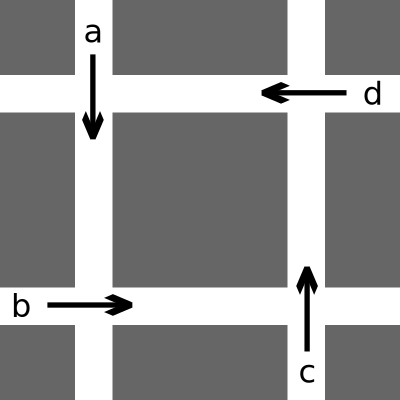
\includegraphics[width=3cm]{img/rightOfWay}
	\caption{Vorfahrt ist nicht transitiv: d hat Vorfahrt vor c hat Vorfahrt vor b hat Vorfahrt vor a hat Vorfahrt vor d}
	\label{fig:rightOfWayNotTransitive}
\end{figure}

Ein Problem beim Überschreiben ist jedoch, dass 'Stummel' vorheriger Markierungen übrig bleiben können, wie in Abb. \ref{fig:overwritingCanCauseStubs} exemplarisch dargestellt. Daher müssen, wenn eine Markierung eines Fahrzeugs entfernt wird, alle Markierungen des Fahrzeugs entfernt werden. Später sind dann die Markierungen des Fahrzeuges neu zu bestimmen.
\begin{figure}[h!]
	\centering
	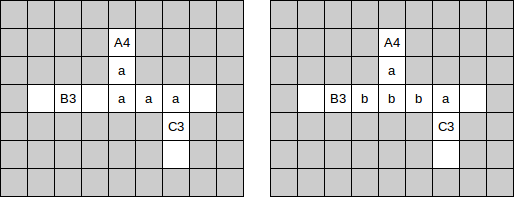
\includegraphics[width=6cm]{img/stubs}
	\caption{Möglichkeit von Stummeln: Links: A markiert zunächst 4 Felder. Dann rechts: B hat vorfahrt, markiert dabei 3 Felder und überschreibt Markierungen von A. Übberreste der Markierungen von A behindern nun C, der eigentlich fahren könnte}
	\label{fig:overwritingCanCauseStubs}
\end{figure}

Zuletzt muss noch das Einhalten von Geschwindigkeitsbegrenzungen gewährleistet werden. Dazu wird jede Zelle mit einer Maximalgeschwindigkeit versehen. Betritt ein Fahrzeug eine Zelle, wird die maximale Anzahl an Zellen, die es darüber hinaus noch markieren kann, auf die Maximalgeschwindigkeit der Zelle gedeckelt. Somit ist gewährleistet, dass kein Fahrzeug an keiner Zelle die zulässige Geschwindigkeit überschreitet.

\subsubsection{Verfahren}
\label{subsubsec:kreisverkehrUmsetzungVerfahren}

Die oben beschriebenen Überlegungen führen zu folgendem Markierungsalgorithmus:
\lstinputlisting{src/streetMapMarkAlgorithm}
wobei r die verbleibenden Schritte des Autos runterzählt. Ob ein Fahrzeug an einer Zusammenführung Vorfahrt hat, ergibt sich wie oben beschrieben aus der Reihenfolge der Vorgängerverweise. Um die Implementierung zu vereinfachen beschränken wir uns auf Zusammenführungen mit zwei Vorgängern.

Nachdem die Markierungen entsprechend gesetzt wurden müssen im Anschluss daran aus ihnen die tatsächlichen Fahrdistanzen für die einzelnen Fahrzeuge berechnet werden. Dazu kann man in jedem Fahrzeug starten und seine Wunschstrecke solange ablaufen, wie man dabei nur vom Fahrzeug markierte Zellen betritt. Hierbei zählt man eine Variable hoch, die am Ende die Geschwindigkeit des Fahrzeuges angibt. Dies geschieht folgendermaßen:\\

\lstinputlisting{src/streetMapDistAlgorithm}

Damit haben wir einen Algorithmus erreicht, der beliebige Verkehrsnetze kollisionsfrei unter Berück\-sichtigung von Vorfahrtsregeln und Geschwindigkeitsbegrenzungen simulieren kann. Im Kontrast zur mehrspurigen Simulation oben kann dieses Verfahren zwar ebenfalls mit mehreren Spuren umgehen, das Rechtsfahrgebot und das Rechtsüberholverbot müssten aber separat implementiert werden. Bis auf das modifizierte Verfahren zur Bestimmung der maximalen Fahrdistanz können die Regeln des Nagel-Schreckenberg Modells \cite{nagel-schreckenberg} übernommen werden. Es werden also zunächst alle Fahrzeuge beschleunigt, dann die Distanzen wie oben beschrieben geprüft, anschließend getrödelt und am Ende die Fahrzeuge bewegt.

Eine schöne Eigenschaft dieser Herangehensweise ist, dass wir ohne zusätzlichen Aufwand Quellen und Senken von Fahrzeugen erzeugen können. Als Quelle wird schlicht jede Zelle definiert, die zwar Nachfolger, aber keine Vorgänger hat. Analog ist jede Zelle eine Senke, die Vorgänger, aber keine Nachfolger hat. Jeder Zelle kann darüber hinaus eine Autoerzeugungswahrscheinlichkeit zugeordnet werden, mit der in der Zelle pro Simulationsschritt ein neues Auto entsteht, sofern sie leer ist. Ein Auto, was eine Senke überfährt, wird hingegen entfernt.

Nun bleibt noch die Frage zu klären, wie an einer Verzweigung die Entscheidung zu treffen ist, in welche Richtung ein Fahrzeug fahren soll (vgl. Zeile 7). Konzeptionell wäre es möglich, jedem neu hinzugefügten Fahrzeug ein Ziel zuzuweisen und einen (randomisierten) Pfadfindungsalgorithmus zu nutzen, um die Entscheidungen an Verzweigungen zu treffen. Da Fahrzeuge in der Regel ein festes Ziel haben, wäre dies der realistischste Ansatz. Zur Vereinfachung der Implementierung entscheiden wir uns allerdings dafür, die Entscheidung an jeder Verzweigung zufällig zu treffen, wobei für jede Nachfolgerzelle individuelle Wahrscheinlichkeiten festgelegt werden können. Da wir nur sehr einfache Straßennetze mit wenigen Verzweigungen (die insbesondere nicht verschachtelt sind) betrachten, erachten wir das als eine ausreichend gute Annäherung. Für komplexere Szenarien werden allerdings komplexere Entscheidungssysteme notwendig.

\subsection{Visualisierung}
\label{subsec:visualisierung}
Die Simulationsergebnisse werden nach Abschluss der Simulation in vier Grafiken visualisiert. Für die Autobahn und beliebige Straßenverläufe wie den Kreisverkehr gibt es bei der Visualisierung keine konzeptionellen Unterschiede. Daher wird die Visualisierung an dieser Stelle nur einmal erläutert, auch wenn wegen einiger Programmierdetails zwei Implementierungen vonnöten sind.\\

\begin{figure}[h!]
	\centering
	\begin{subfigure}[b]{0.3\textwidth}
		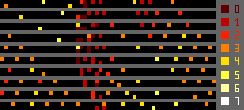
\includegraphics[width=\textwidth]{img/vis_multilane_2_lanes}
		\caption{Momentaufnahmen von zehn Simulationsschritten (Ausschnitt)}
		\label{fig:momentaufnameMultilane}
	\end{subfigure}
	~
	\begin{subfigure}[b]{0.3\textwidth}
		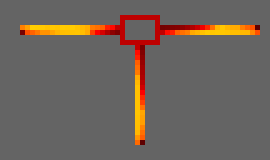
\includegraphics[width=\textwidth]{img/vis_roundabout_speed_heat_map}
		\caption{Geschwindigkeits-Heat-Map eines Kreisverkehrs}
		\label{fig:speedMapRoundabout}
	\end{subfigure}
	~
	\begin{subfigure}[b]{0.3\textwidth}
		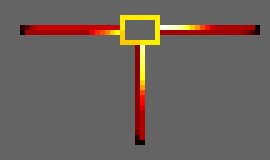
\includegraphics[width=\textwidth]{img/vis_roundabout_occupancy_heat_map}
		\caption{Belegungs-Heat-Map eines Kreisverkehrs}
		\label{fig:occupancyMapRoundabout}
	\end{subfigure}
	\caption{Diverse Visualisierungsmethoden}
	\label{fig:visualizationMethods}
\end{figure}

\paragraph{Momentaufnahme}
\label{paragraph:momentaufnahme}

Nach jedem Simulationsschritt wird eine Momentaufnahme der aktuellen Verkehrssituation gemacht. Dazu wird zunächst eine komplett schwarze Grafik erzeugt, welche genau so groß ist wie die Straßenkarte. Anschließend wird für jedes Fahrzeug gemäß seiner Geschwindigkeit das entsprechende Pixel eingefärbt. Dabei steht die Farbe Dunkelrot für ein stehendes Fahrzeug und die Farbe Weiß für die globale Maximalgeschwindigkeit 7 = 189 $km/h$. Dann wird die aktuelle Momentaufnahme an die bisherigen Momentaufnahmen angefügt. Abbildung \ref{fig:momentaufnameMultilane} zeigt exemplarisch die Momentaufnahmen einer zweispurigen Autobahn über zehn Simulationsschritte hinweg.

Für Simulationen mit vielen Spuren und über viele Simulationsschritte hinweg kann ein solches Bild natürlich sehr hoch werden. Die zwei nachfolgenden Auswertungen sind deutlich kompakter.

\paragraph{Geschwindigkeits-Heat-Map}
\label{paragraph:speedmap}

Die Geschwindigkeits-Heat-Map stellt dar, mit welcher Geschwindigkeit sich Fahrzeuge im Durchschnitt über die einzelnen Zellen bewegt haben. Dazu wird nach jedem Simulationsschritt für jedes Fahrzeug ermittelt, welche Zellen es mit welcher Geschwindigkeit passiert hat.

Die Farben in der Geschwindigkeits-Heat-Map entsprechen denen der Momentaufnahmen, wobei Zellen schwarz werden, wenn dort während der gesamten Simulation kein einziges Fahrzeug entlang fuhr. Bei einer weißen Zelle hatten alle Fahrzeuge, die diese Zelle passiert haben, Geschwindigkeit 7. Im gegebenen Beispiel in Abbildung \ref{fig:speedMapRoundabout} ist deutlich ersichtlich, dass die Geschwindigkeit im Kreisverkehr geringer als auf den Zubringern ist.

\paragraph{Belegungs-Heat-Map}
\label{paragraph:occupancymap}
Die Belegungs-Heat-Map gibt an, während wievieler Schritte eine Zelle von einem Fahrzeug überquert wurde, unabhängig von der Geschwindigkeit. Auf diese Weise können wir ermitteln, wie stark die unterschiedlichen Bereiche eines Straßennetzes ausgelastet waren. Bei der Belegungs-Heat-Map geben die Farben keine Geschwindigkeit an. Während eine schwarze Zelle anzeigt, dass sich hier zu keinem Zeitpunkt ein Fahrzeug befand, war eine weiße Zelle durchgängig belegt.

\paragraph{Verkehrsdichte}
\label{paragraph:verkehrsdichte}

Bei einer Simulation mit periodischen Randbedingungen ist die Verkehrsdichte konstant, mit offenen Randbedingungen kann sie jedoch durchaus aufschlussreich sein. Daher wird nach der Simulation eine Grafik erzeugt, die zu jedem Simulationsschritt die dazugehörige Verkehrsdichte anzeigt.
\begin{figure}[h!]
	\centering
	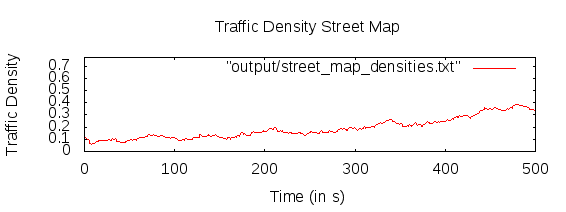
\includegraphics[width=0.9\textwidth]{img/vis_street_map_densities}
	\caption{Belegungs-Heat-Map eines Kreisverkehrs}
	\label{fig:trafficDensityMapRoundabout}
\end{figure}


\section{Ergebnisse}
\label{sec:ergebnisse}

\subsection{Einspurige Autobahn}
\label{subsec:einspurig}

Gemäß unseren Erwartungen konnten wir feststellen, dass es mit einem Trödelfaktor von 0 auf einer 2,25$km$ langen einspurigen Autobahn nur unter ungünstigen Bedingungen zu Staus kommt. Gehen wir davon aus, dass alle Fahrzeuge auf der Autobahn eine Maximalgeschwindigkeit von 7 haben und dass die Fahrzeuge bei periodischen Randbedingungen äquidistant und mit ihrer Maximalgeschwindigkeit auf der Fahrbahn platziert werden, dann haben die Fahrzeuge bei ausreichend geringer Verkehrsdichte stets genug Platz, um ungehindert vorwärts zu fahren. Wird die Verkehrsdichte erhöht, müssen die Fahrzeuge aufgrund des Platzmangels abbremsen. Es kommt jedoch nicht zu Staus. Zum Stillstand kommt es erst, wenn alle Zellen mit Fahrzeugen besetzt sind.

Wird statt einer äquidistanten eine zufällige Initialisierung verwendet und haben die Fahrzeuge alle unterschiedliche Initialgeschwindigkeiten, kommt es aufgrund ungünstiger Fahrzeugplatzierungen anfangs zu Staus. Bei geringen Verkehrsdichten wie 0.1 lösen sich diese innerhalb weniger Iterationen komplett auf, bei höheren Verkehrsdichten kommt es jedoch dazu, dass einige Fahrzeuge aufgrund der Verkehrsdichte nicht ausreichend Platz haben, um mit ihrer Maximalgeschwindigkeit zu fahren. Daher kommt es zu Staus, deren Anzahl von der Höhe der gewählten Verkehrsdichte abhängt. Diese Staus haben das Charakteristikum, dass sie sich immer weiter nach hinten (bzw. links) entwickeln und sich niemals komplett auflösen.

Falls wir eine Simulation ohne periodische Randbedingungen durchführen und Fahrzeuge nur am linken Rand der Autobahn erzeugt werden, ist es unmöglich, gewisse Verkehrsdichten zu erreichen. Die Abbildung \ref{fig:ergEinspurigKeinWraparoundKeinStau} illustriert diesen Sachverhalt.

\begin{figure}[h!]
	\centering
	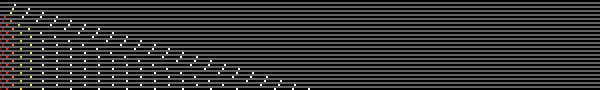
\includegraphics[width=\textwidth]{img/erg_einspurig_kein_wraparound_dichte_0_5}
	\caption{Staufreiheit bei Simulation ohne periodische Randbedingungen}
	\label{fig:ergEinspurigKeinWraparoundKeinStau}
\end{figure}

Während das erste Fahrzeug noch umgehend auf seine Maximalgeschwindigkeit beschleunigen kann, muss das zweite Fahrzeug seine Geschwindigkeit eins niedriger wählen, denn das erste Fahrzeug blockiert die letzte Zelle, die das neue Fahrzeug befahren möchte. Dieser Effekt setzt sich immer weiter fort, bis ein neu erzeugtes Fahrzeug sich nicht einmal eine Zelle weit bewegen kann. Da nur in der ersten Zelle der Fahrbahn neue Fahrzeuge erzeugt werden können, wird nun nur in jeder zweiten Runde ein Fahrzeug erzeugt. Somit sind hohe Verkehrsdichten mit diesem Modell nicht umsetzbar und es muss auf den Ansatz mit den periodischen Randbedingungen zurückgegriffen werden. Im Folgenden wird daher ausschließlich dieser Ansatz verwendet.

Als nächstes betrachten wir randomisierte Maximalgeschwindigkeiten. In diesem Szenario weichen die Ergebnisse nur in sofern von den bisherigen Ergebnissen ab, dass nach einigen Iterationen alle Fahrzeuge mit der Maximalgeschwindigkeit des langsamsten Fahrzeuges fahren. Natürlich gilt dies nur, solange die Verkehrsdichte nicht zu hoch gewählt wird. Im Folgenden werden wir die Auswirkungen des Trödelfaktors untersuchen. Um die Ergebnisse möglichst frei von anderen Einwirkungen zu halten, erhalten ab jetzt alle Fahrzeuge eine Maximalgeschwindigkeit von 7.

Wir nehmen eine Verkehrsdichte von 0.1 und äquidistante Initialisierung an. Bei Trödelfaktoren zwischen 0.05 und 0.15 treten noch keine Staus auf, alle Fahrzeuge fahren größtenteils ungehindert mit ihrer Maximalgeschwindigkeit. Erhöhen wir die Trödelfaktoren auf Werte zwischen 0.1 und 0.2 kommt es gelegentlich zu lokal beschränkten Geschwindigkeitsreduktionen, die jedoch nicht in einem wirklichen Stau resultieren. Setzen wir das Trödelfaktorintervall auf 0.15 bis 0.25, kommt es zuweilen zu Staus aus dem Nichts. Abbildung \ref{fig:ergStauAusDemNichtsP0_2} illustriert wie aus einer unkritischen Verkehrslage ein Stau entsteht. Dadurch dass ein Fahrzeug zufällig seine Geschwindigkeit mehrmals nacheinander reduziert, müssen die nachfolgenden Fahrzeuge ebenfalls bremsen. Bei Trödelfaktoren auf diesem Niveau lösen sich die Staus jedoch zumeist nach einigen Iterationen auf.

\begin{figure}[h!]
	\centering
	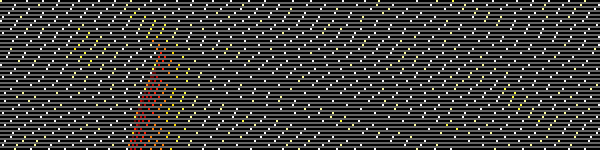
\includegraphics[width=\textwidth]{img/erg_einspurig_stau_aus_dem_nichts_dichte_0_1_p_0_15_bis_0_25}
	\caption{Stau aus dem Nichts bei Trödelfaktoren zwischen 0.15 und 0.25}
	\label{fig:ergStauAusDemNichtsP0_2}
\end{figure}

Bei Trödelfaktoren zwischen 0.2 und 0.3 hingegen bestehen Staus manchmal sogar über etwa eintausend Iterationen hinweg, sie lösen sich nur noch gelegentlich in angemessener Zeit auf. Ab Trödelfaktoren zwischen 0.25 und 0.35 lösen sich einmal gebildete Staus selbst über Simulationen über 2000 Sekunden nicht mehr auf. %\textcolor{AI-BLUE}{Bis zu Trödelfaktoren zwischen 0.45 und 0.55 ist die Autobahn bei zumeist einem größeren Stau noch halbwegs befahrbar, mit höheren Faktoren können nur vereinzelt Fahrzeuge kurze Strecken zurücklegen, ohne in einen Stau zu kommen.}

Wählen wir eine zufällige Initialisierung, kommt es bereits bei Trödelfaktoren von 0.1 bis 0.2 zu Staus, die sich in der Regel nicht mehr auflösen. Dies entspricht dem Verhalten bei äquidistanter Initialisierung mit Trödelfaktoren zwischen 0.2 und 0.3.
Bei der Verkehrsdichte 0.15 und sowohl zufälliger als auch äquidistanter Initialisierung genügen bereits sehr kleine Trödelfaktoren zwischen 0 und 0.05, um permanente Staus zu verursachen. Höhere Verkehrsdichten verstärken die aufgeführten Effekte.

\subsection{Mehrspurige Autobahn}
\label{subsec:mehrspurig}

Um nur die Auswirkungen der rücksichtsvollen Fahrstreifenwechsel bei variierenden Verkehrsdichten, äquidistanter Initialisierung und auf 7 konzentrierten Maximalgeschwindigkeiten analysieren zu können, setzen wir zunächst den Trödelfaktor auf den Wert 0 (Minimalwert = Maximalwert = 0) und die Risikobereitschaft der Fahrzeuge auf praktisch 0, indem wir als Lambda für die Exponentialverteilungen der Risikofaktoren den Wert 10'000 wählen.
Anders als bei der einspurigen Autobahn beginnen wir bei der Betrachtung der zweispurigen Autobahn mit einer Vekehrsdichte von 0.05. Die Gesamtanzahl der Fahrzeuge entspricht in diesem Szenario der Anzahl der Fahrzeuge auf einer einspurigen Autobahn bei einer Verkehrsdichte von 0.1.
In diesem Szenario kann die Verkehrsdichte auf 0.08 erhöht werden, ohne dass es grundsätzlich zu nennenswerten Geschwindigkeitsreduktionen kommt. Bei höheren Verkehrsdichten wie 0.1 oder 0.125 müssen wir jedoch das Auftreten zahlreicher, sich nicht auflösender Staus konstatieren.
Während es also auf der einspurigen Autobahn bei äquidistanter Initialierung unabhängig von der Verkehrsdichte nie zu Staus kommt, sondern nur zu gleichmäßigen, kollektiven Geschwindigkeitsreduktionen, führt bei nah hintereinander fahrenden Fahrzeugen der Abbremszwang des rechten, hinteren Fahrzeuges dazu, dass sich die Geschwindigkeiten der Fahrzeuge nicht an allen Stellen der Autobahn gleichmäßig reduzieren, sondern an manchen Stellen mehr Rückstaus auftreten als an anderen. Zwar fahren die Fahrzeuge im Schnitt nicht zwangsweise langsamer, sie müssen ihre Geschwindigkeit jedoch häufiger an die aktuelle Verkehrslage anpassen.

Bei einer Verkehrsdichte von 0.08 und händisch auf exakt 0 gesetzten Risikofaktoren erhöhen wir nun schrittweise den Trödelfaktor, um allein dessen Einfluss untersuchen zu können.Es lässt sich feststellen, dass es bereits bei Werten aus dem Intervall von 0 bis 0.01 zu Staus aus dem Nichts kommt. Bei einem Trödelfaktor von 0 optimieren sich die Abstände zwischen den Fahrzeugen nach einigen Schwierigkeiten nach der Initialisierung und alle Fahrzeuge können mit ihrer Maximalgeschwindigkeit weiter fahren. Wird jedoch der Trödelfaktor auch nur leicht angehoben, kommt es zu Situationen wie im letzten Abschnitt beschrieben. Es müssen also Fahrzeuge auf dem rechten Fahrstreifen ihre Geschwindigkeit drastisch reduzieren, was zu Rückstaus führt.

\begin{figure}[h!]
	\centering
	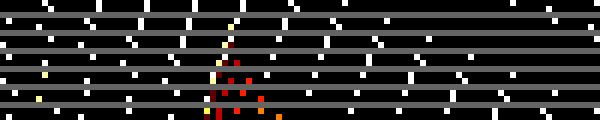
\includegraphics[width=\textwidth]{img/erg_mehrspurig_stau_aus_dem_nichts_p_0_01}
	\caption{Stau aus dem Nichts bei Trödelfaktoren zwischen 0 und 0.01}
	\label{fig:ergStauAusDemNichtsMehrspurigP0_01}
\end{figure}

Abbildung \ref{fig:ergStauAusDemNichtsMehrspurigP0_01} zeigt eine solche Situation. In der ersten Momentaufnahme fahren acht Fahrzeuge je zweit nebeneinander. Beim zweiten dieser Paare reduziert das rechtsfahrende Fahrzeug seine Geschwindigkeit um eine Stufe und muss daher aufgrund des Rechtsüberholverbots seine Geschwindigkeit auf 0 reduzieren, was schlussendlich in einem Stau resultiert. Höhere Trödelfaktoren verstärken erwartungsgemäß die Intensität und die Anzahl der auftretenden Staus.

Belassen wir es nun bei einem Trödelfaktor von 0 und erhöhen die Risikofaktoren. Bei einem Lambda von 32 für beide Risikofaktoren erhalten wir einen Mittelwert von $\frac{1}{32}$ und einen Maximalwert von 0.10958. In einem solchen Szenario kommt es zu Situation wie in Abbildung \ref{fig:ergStauAusDemNichtsMehrspurig_p_0_r_32}. Das violett umkringelte Fahrzeug zieht, ohne auf Abstände zu achten, auf die linke Spur herüber. Das blau umkringelte Fahrzeug muss daraufhin seine Geschwindigkeit stark reduzieren, wodurch es zu einem Stau kommt.

\begin{figure}[h!]
	\centering
	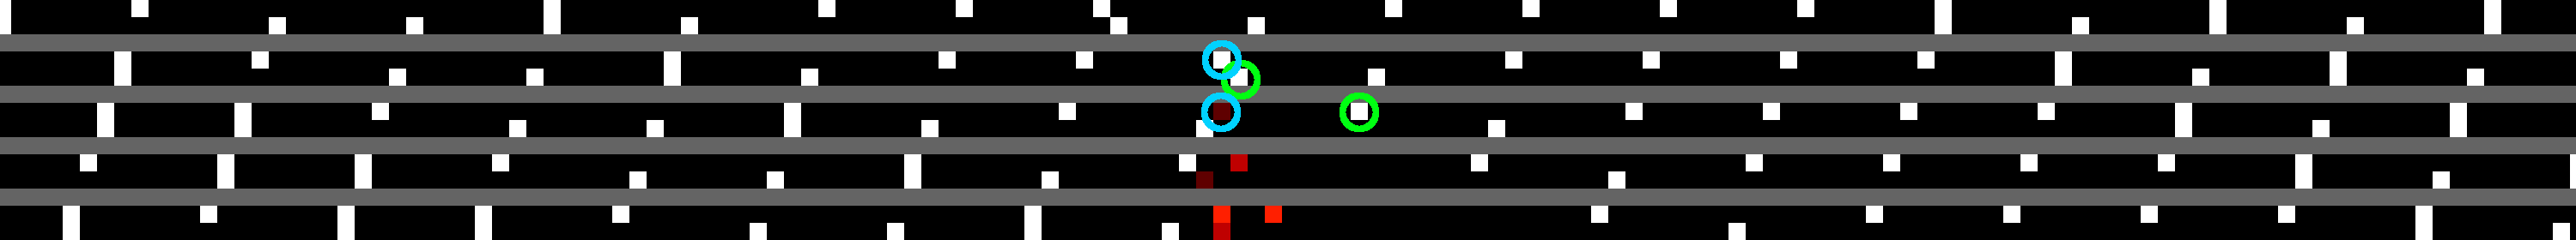
\includegraphics[width=\textwidth]{img/erg_mehrspurig_stau_wegen_risikospurwechsel_p_0_r_32_version2}
	\caption{Stau aus dem Nichts bei Trödelfaktor 0 und $\lambda_{L2R} = \lambda_{R2L} = 32$}
	\label{fig:ergStauAusDemNichtsMehrspurig_p_0_r_32}
\end{figure}

Interessanterweise ist es das System gegenüber Risikofahrstreifenwechseln bemerkenswert robust. Selbst bei sehr hohen Risikofaktoren (z.B. mit $\lambda = 2$) kommt es nur zu Beginn der Simulation zu Staus. Nach und nach lösen sich die Staus auf, wobei zufallsbedingt immer mehr Fahrzeuge direkt nebeneinander fahren. Da wir nicht trödeln, ist es nicht möglich, eine solche Konstellation wieder zu verlassen. Weil somit die direkte Nachbarzelle stets belegt ist, können immer weniger Fahrzeuge die Spur wechseln. Irgendwann ist das System so stabil, dass keine Staus mehr auftreten. Diesem Szenario muss man allerdings die Plausibilität absprechen. Dass alle Fahrzeuge über längere Zeit parallel fahren, ist realitätsfern.

Kombiniert man Trödeln und Risikofahrstreifenwechsel erhöht sich die Anzahl und Intensität mit steigendem Trödelfaktor und sinkenden Lambda-Werten für die beiden Risikofaktorexponentialverteilungen. Wählt man das Intervall von 0.2 bis 0.3 für den Trödelfaktor und $\lambda_{L2R} = \lambda_{R2L} = 8$ zur Bestimmung der Risikofaktoren erhöht sich die Anzahl und Intensität der Staus drastisch. Der in Abbildung \ref{fig:ergMehrspurigTroedelnUndRisikowechsel} gezeigte Ausschnitt einer langen Simulation verdeutlicht diesen Umstand.

\begin{figure}[h!]
	\centering
	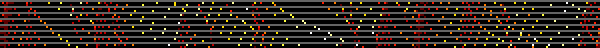
\includegraphics[width=\textwidth]{img/erg_mehrspurig_troedeln_und_risikowechsel}
	\caption{Schleichender Verkehr bei Kombination von Trödeln und Risikofahrstreifenwechsel}
	\label{fig:ergMehrspurigTroedelnUndRisikowechsel}
\end{figure}

All diese Ergebnisse gelten für eine Verkehrsdichte von 0.08. Höhere Verkehrsdichten verstärken die aufgeführten Effekte deutlich.


\subsection{Kreisverkehr}
\label{subsec:kreisverkehr}
Bei der Simulation des Verkehrsflusses an einem Kreisverkehr gibt es Verzweigungen und Zusammenführungen, wobei Vorfahrtsregeln und Geschwindigkeitsbegrenzungen zu beachten sind. Daher wird das in Abschnitt \ref{subsec:umsetzung-kreisverkehr} entwickelte Verfahren benutzt. Simuliert wird ein Kreisverkehr mit \texttt{8 Zellen Breite} und \texttt{6 Zellen Höhe}, es handelt sich also näherungsweise um ein Rechteck mit \texttt{60m} Breite und \texttt{45m} Höhe, da wir weiterhin von einer Zellenlänge von $7.5m$ ausgehen. Zum Kreisverkehr führen \texttt{3 Zubringerstraßen bzw. Ausfahrten} die von links, rechts und unten kommen, dementsprechend gibt es \texttt{3 Quellen} und \texttt{3 Senken}. An der Oberseite befinden sich keine Abzweigungen, der Kreisverkehr weist also eine Asymmetrie auf. Die Länge der Zu- und Abfahrten kann variiert werden. Wir entschließen uns dazu, sie auf \texttt{20 Zellen} zu setzen. Zusätzlich gilt die Forderung, dass Fahrzeuge nur mit einer Geschwindigkeit von \texttt{einer Zelle pro Sekunde} in den Kreisverkehr einfahren dürfen, was einer Realgeschwindigkeit von $27km/h$ entspricht. Aufgrund der Proportionen des Kreisverkehrs erscheint es uns auch angemessen, die Geschwindigkeit innerhalb des Kreisverkehrs auf diesen Wert zu beschränken. Da wir von einer Landstraße ausgehen setzen wir das Limit für die Zu- und Abfahrten auf \texttt{4 Zellen/Sekunde}, was $108km/h$ entspricht. Damit ergibt sich die in Abbildung \ref{fig:roundaboutSmall} zu sehenden schematische Darstellung der Straßenkarte.

\begin{figure}[h!]
	\centering
	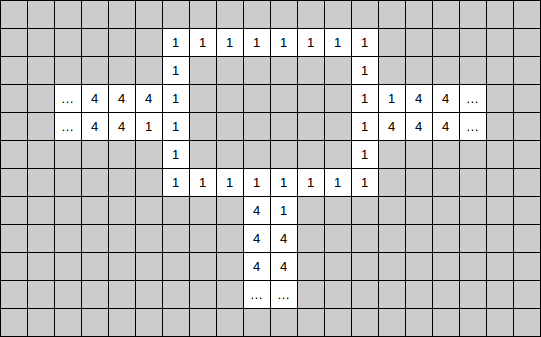
\includegraphics[width=6cm]{img/roundaboutSmall}
	\caption{Kreisverkehr mit eingetragenen Höchstgeschwindigkeiten}
	\label{fig:roundaboutSmall}
\end{figure}

Schließlich müssen wir noch die Wahrscheinlichkeit, den Kreisverkehr an jeder der Verzweigungen zu verlassen, definieren. Diese wird auf \texttt{1/3} gesetzt, was dazu führt, dass die Wahrscheinlichkeit, die erste oder die zweite Ausfahrt zu nehmen näherungsweise gleich ist, bei der dritten Ausfahrt (wo das Fahrzeug hergekommen ist) aber signifikant geringer.

Mit diesen Parametern lässt sich beobachten, dass sich ab einer \texttt{car generation rate von etwa 0.15} Rückstaus auf dem Zufahrten bilden die mal wachsen, mal schrumpfen. Die car generation rate ist dabei die Wahrscheinlichkeit, mit der an jeder der Quellen unabhängig voneinander ein Fahrzeug hinzugefügt wird. Da wir 3 Quellen haben bedeutet dies, dass in jedem Simulationsschritt im Schnitt $0.45$ Autos den Simulationsbereich betreten. Für niedrigere Werte bilden sich keine Rückstaus, für höhere sind sie nahezu garantiert und wachsen stetig.

Dazu wollen wir uns exemplarisch die Ergebnisse für eine Erzeugungsrate von $0.10$ ansehen, wobei in jeder Runde in etwa $3 \cdot 0.10 = 0.30$ Fahrzeuge die Simulation betreten, also etwa ein Auto in jedem dritten Simulationsschritt. Abbildung \ref{fig:roundabout010} zeigt einen typischen Zustand des Kreisverkehrs nach 500 Iterationen.

\begin{figure}[h!]
	\centering
	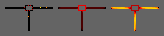
\includegraphics[width=\textwidth]{img/roundabout_010}
	\caption{Erzeugungsrate 0.10. Links: Kreisverkehr nach 500 Iterationen, Mitte: Belegungshäufigkeit, Rechts: Durchschnittsgeschwindigkeit}
	\label{fig:roundabout010}
\end{figure}

Man kann beobachten, dass im Kreisverkehr selbst die Dichte etwas höher ist als an den Auf- und Abfahrten, es ist aber noch genügend Platz für ankommende Autos, die ebenfalls in den Kreisverkehr wollen. Im mittleren Bild sieht man die Belegungshäufigkeit der einzelnen Zellen, und es wird deutlich dass der Kreisverkehr die am intensivsten genutzte Region ist. Dies ist naheliegend, da alle Fahrzeuge diese Region passieren müssen, jede Zufahrtsstraße aber nur von einem Drittel der Autos genutzt wird. Die Durchschnittsgeschwindigkeit in jeder Zelle lässt sich dem rechten Bildteil entnehmen, wobei man sieht dass auf den Zufahrtsstraßen die Durchschnittsgeschwindigkeit der Maximalgeschwindigkeit 4 entspricht. Vom Kreisverkehr bzw. den Quellen weg wird auf diesen Wert beschleunigt. Bei der Anfahrt auf den Kreisverkehr kann es zuweilen vorkommen, dass man auf eine Einfahrmöglichkeit warten muss, weswegen sich die Geschwindigkeit graduell verlangsamt je näher man kommt.

Das Verhalten des Systems über die Zeit zeigt die Abbildung \ref{fig:roundabout010density}, in der die Verkehrsdichte gegen die Zeit in Simulationsschritten abgetragen ist. Sie ist merklichen Schwankungen unterworfen, die sich aus dem Herausfahren von Fahrzeugen und dem zufälligen Neuerzeugen ergeben. Sie bleibt aber etwa mit 0.14 nach oben beschränkt, was zeigt dass der Verkehr flüssig fahren kann.

\begin{figure}[h!]
	\centering
	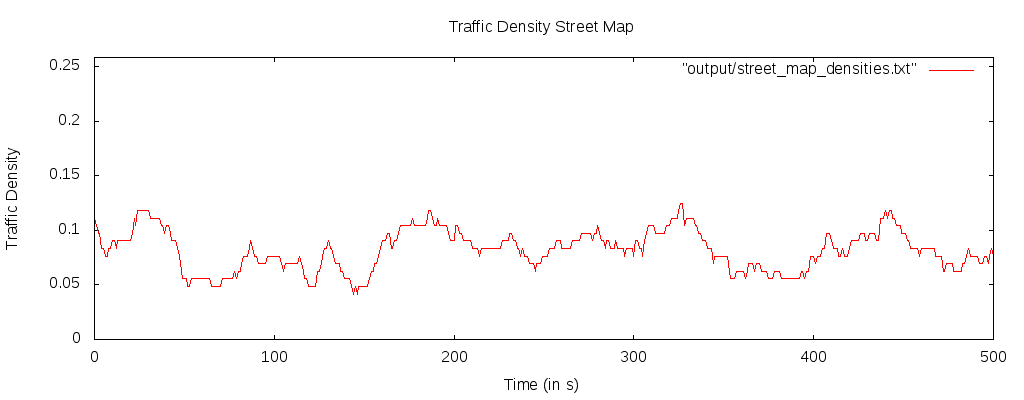
\includegraphics[width=\textwidth]{img/roundabout_010_densities}
	\caption{Dichte im Kreisverkehr über 500 iterationen bei Erzeugungsrate 0.10}
	\label{fig:roundabout010density}
\end{figure}

Erhöhen wir die Erzeugungsrate auf 0.20, so zeigt sich ein anderes Bild. Es betreten nun in jedem Simulationsschritt im Mittel etwa $3 \cdot 0.20 = 0.60$ Fahrzeuge, also etwas mehr als ein halbes, die Simulation. Die dazugehörigen Messwertbilder sind in Abbildung \ref{fig:roundabout020} zu sehen und unterscheiden sich deutlich von denen für eine Erzeugungsrate von 0.10.

\begin{figure}[h!]
	\centering
	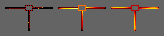
\includegraphics[width=\textwidth]{img/roundabout_020}
	\caption{Erzeugungsrate 0.20. Links: Kreisverkehr nach 500 Iterationen, Mitte: Belegungshäufigkeit, Rechts: Durchschnittsgeschwindigkeit}
	\label{fig:roundabout020}
\end{figure}

Zunächst fällt auf dass der Kreisverkehr komplett gefüllt ist. Da sich die Fahrzeuge im Kreis alle mit Geschwindigkeit 1 bewegen und Vorfahrt haben sind in jeder Runde alle Felder belegt. Da auf den Zufahrtsstraßen aber weiterhin Fahrzeuge ankommen bildet sich hier ein Rückstau, der Stellenweise Lücken aufweist wo Autos einem in den Kreis eingefahrenen nachrücken. Dies zeigt sich auch an der Belegungshäufigkeit der Zellen, die auf den Zufahrtsstraßen nun wesentlich höhere Werte annimmt. Wo vormals eine in etwa gleiche Nutzung von Zu- und Abfahrtsstraßen zu sehen war tritt nun eine starke Diskrepanz auf, wobei die Auslastung im Kreisverkehr weiterhin hoch ist. Die Durchschnittsgeschwindigkeiten sind dementsprechend geringer. Während innerhalb des Kreisverkehrs aufgrund der Vorfahrt eine Zelle vor jedem Fahrzeug frei bleibt und des dementsprechend nicht zu systematischen Staus kommt stehen die Fahrzeuge auf den Zufahrtsstraßen über weite Teile der Strecke und müssen warten, bis der Vorderste in den Kreisverkehr einfahren kann. Fahrzeuge, die die Abfahrtsstraßen erreichen können ungehindert beschleunigen, da sie in der Regel keine Autos vor sich haben.

\begin{figure}[h!]
	\centering
	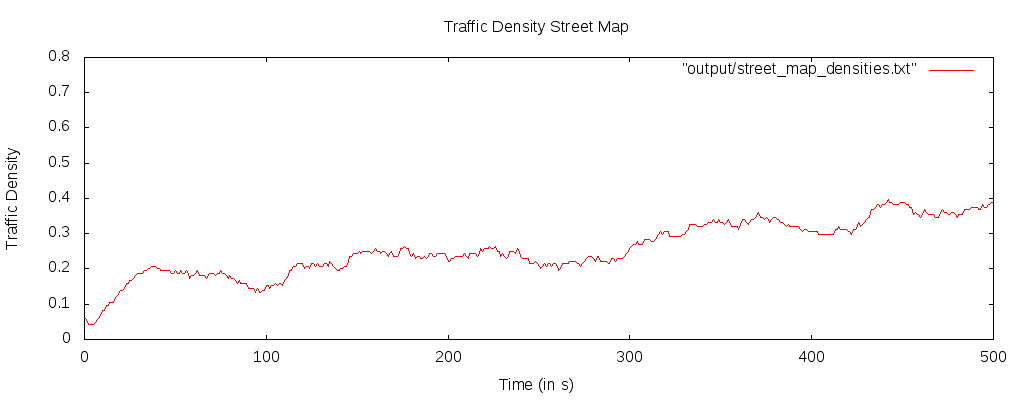
\includegraphics[width=\textwidth]{img/roundabout_020_densities}
	\caption{Dichte im Kreisverkehr über 500 iterationen bei Erzeugungsrate 0.20}
	\label{fig:roundabout020density}
\end{figure}

Der Verlauf der Verkehrsdichte zu diesem Durchlauf ist in Abbildung \ref{fig:roundabout020density} dargestellt. Zu Beginn der Simulation befinden sich nur wenige Fahrzeuge auf der Strecke, dieser Wert steigt allerdings durch die ankommenden Fahrzeuge kontinuierlich, und erreicht dabei eine Dichte von etwa $0.4$. Dies entspicht dem Zeitpunkt, ab dem aus Platzgründen keine Fahrzeuge mehr an den Quellen generiert werden können bis ein Fahrzeug den Kreisverkehr verlässt und andere nachrücken können.

\subsection{Autobahndreieck}
Ein Vorzug des entwickelten Algorithmus ist seine Allgemeingültigkeit. Er lässt sich ohne problemspezifische Anpassungen auf beliebige Straßennetze anwenden, sogar auf nicht-planare. Daher sind wir ebenfalls in der Lage, den Verkehrsfluss an einem Autobahndreieck zu simulieren, wobei wir uns für die Bauform \q{Trompete} mit Linksführung entscheiden.

\begin{figure}[h!]
	\centering
	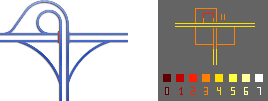
\includegraphics[width=8cm]{img/interchangeTrumpetSpeedLimits}
	\caption{Autobahndreieck. Links: Schematische Darstellung \cite{wiki:trumpetInterchange}, Rechts: Umsetzung mit Maximalgeschwindigkeiten}
	\label{fig:interchangeTrumpet}
\end{figure}

Hierbei nehmen wir auf den Autobahnen ein Tempolimit von 4 (also $108km/h$) in der Nähe des Dreiecks an. Für die Verbindungsstraßen werden Limits von 3 ($81km/h$) bzw. 2 ($54km/h$) entsprechend ihrer Krümmung ausgewählt. Da die von unten kommende Autobahn unter (oder über) der anderen verlaufen muss und damit die selben Zellen nutzen würde, wäre diese Formation mit regulären zellulären Automaten nicht darstellbar. In der Repräsentation als Graph, auf der unser Algorithmus arbeitet, ist dies jedoch kein Problem. Zur graphischen Aufbereitung platzieren wir das Unterführungsstück isoliert abseits der anderen Straßen, wie in Abbildung \ref{fig:interchangeTrumpet} zu sehen ist.

Ebenso wie der Kreisverkehr verfügt dieses System über 3 Quellen und 3 Senken, verhält sich unter hoher Verkehrslast allerdings wesentlich zuverlässiger. Selbst bei einer Erzeugungsrate von $1.00$, wenn also wann immer möglich ein Fahrzeug eingefügt wird, kommt es nicht zu permanenten Staus.

\begin{figure}[h!]
	\centering
	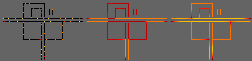
\includegraphics[width=\textwidth]{img/interchangeTrumpet_100}
	\caption{Erzeugungsrate 1.00. Links: Autobahndreieck nach 500 Iterationen, Mitte: Belegungshäufigkeit, Rechts: Durchschnittsgeschwindigkeit}
	\label{fig:interchangeTrumpet100}
\end{figure}

Abbildung \ref{fig:interchangeTrumpet100} visualisiert das Autobahndreieck mit dieser Erzeugungsrate nach 500 Iterationen, wobei dieselben Parameter wie beim Kreisverkehr in Abschnitt \ref{subsec:kreisverkehr} verwendet wurden. Die Zufahrtsstraßen haben sich mit Autos gefüllt, deren Abstände ungefähr der zulässigen Maximalgeschwindigkeit entsprechen. An der in der Mitte dargestellten Belegung lässt sich erkennen, dass es auf den Verbindungsstraßen und den Autobahnstrecken zwischen den Auf- und Abfahrten weniger Fahrzeuge gibt, was naheliegend ist, da sie sich auf Verbindungsstraßen sowie Auf- und Abfahrten aufteilen. Die Geschwindigkeiten im rechten Bild entsprechen ungefähr den Maximalgeschwindigkeiten, wobei es nahe an den Zusammenführungen zu Veringerungen der Geschwindigkeit kommt, Stauketten bilden sich allerdings keine.

\section{Fazit}
\label{sec:fazit}

Zur Simulation von Autobahnen wurde ein auf Zellularautomaten basierendes System entwickelt, welches grundsätzlich mit beliebig vielen Spuren umgehen kann. Für die einspurige Autobahn hat sich ergeben, dass zur Stauvermeidung die äquidistante Initialisierung der zufälligen vorzuziehen ist. Darüber hinaus wurde konstatiert, dass es zur Beibehaltung hoher Verkehrsdichten notwendig ist, den Simulationsansatz mit periodischen statt offenen Rahmenbedinungen zu wählen. Es hat sich ergeben, dass randomisiert bestimmte Maximalgeschwindigkeiten allgemein zu langsamer fahrenden Fahrzeugen führen. Um den Einfluss der anderen Effekte besser untersuchen zu können, wurde die Maximalgeschwindigkeit für alle Fahrzeuge auf 7 festgesetzt. Für eine Verkehrsdichte von 0.1 wurde festgestellt, dass es ab Trödelfaktoren aus dem Intervall von 0.15 bis 0.25 zu Staus aus dem Nichts kommt.

Bei der zweispurigen Autobahn sind kleinere Verkehrsdichten als bei der einspurigen Autobahn notwendig. Bei Idealbedingungen (äquidistante Initialisierung, gleiche Maximalgeschwindigkeiten, Trödelfaktor 0 und ausgesprochen niedrige Risikofaktoren) gewährleistet eine Verkehrsdichte von 0.08 einen größtenteils reibungslosen Verkehrsfluss (dies sind 1.6 mal so viele Fahrzeuge wie bei einer Spur mit Verkehrsdichte 0.1). Kam es auf der einspurigen Autobahn unter ähnlichen Bedingungen zu kollektiven Geschwindigkeitsreduktionen, entstanden bei zwei Spuren aufgrund des Rechtsüberholverbots lokale Rückstaus. Staus aus dem Nichts entstanden bereits bei sehr niedrigen Trödelfaktoren zwischen 0 und 0.01. Höhere Trödelfaktoren erhöhen die Anzahl und Intensität der Staus entsprechend. Der Einfluss der Risikofaktoren hat sich als überraschend gering herausgestellt. Zwar führen Risikofahrstreifenwechsel zuweilen zu Staus, der Einfluss des Trödelfaktors kann allerdings als deutlich größer angesehen werden. Kombinationen von Trödeln und Risikofahrstreifenwechseln führen ebenso wie höhere Verkehrsdichten zu längeren und zahlreicheren Staus. 

Für den Kreisverkehr und beliebige andere Straßennetze, auch nicht-planare, konnten wir ein Verfahren finden, dass bei gewährleisteter Kollisionsfreiheit Vorfahrtsregeln und Tempolimits einhält. Die zentralen Ideen dabei sind ein zusätzlicher Markierungsschritt für abzufahrende Straßenteile und das Herunterzählen der verbleibenden Bewegungsschritte. Anschließend werden die Markierungen gezählt und bilden damit die neue Geschwindigkeit des Fahrzeugs. Unsere Implementierung nutzt ein randomisiertes Verfahren zur Richtungsfindung der Fahrzeuge, was für die betrachteten Szenarien ausreichend ist. In komplexeren Systemen, insbesondere solchen mit vielen Kreisen, muss allerdings ein nahezu ewiges Im-Kreis-Fahren der Fahrzeuge unterbunden werden. Mit diesem Verfahren konnten wir ermitteln, dass für den betrachteten Kreisverkehr die kritische Zuflussrate an Fahrzeugen pro Quelle und Schritt etwa bei $0.15$ liegt. Für das Autobahndreieck lassen sich mit plausiblen Parametern keine Staus erzeugen, wobei zu beachten ist, dass die Zuflussrate durch die offenen Randbedingungen strukturell begrenzt ist.

%\blindtext asdf \cite{mehrspurig}\\
%In Kapitel \myref{sec:einleitung} steht Shit. In Foobar (\myrefcomma{sec:ansatz}) bla

\addcontentsline{toc}{section}{Literatur}
\bibliography{ref}{}
\bibliographystyle{alpha}

\end{document}